\documentclass{report}
\usepackage[parfill]{parskip}
\usepackage{todonotes}
\usepackage{hyperref}
\usepackage{amsmath}
\usepackage{wrapfig}
\usepackage{graphicx}
\usepackage{fancyvrb}
\usepackage{textcomp}
\usepackage{bytefield}
\graphicspath{ {./img/} }
\begin{document}

\title{NEA: Font Rasterizer}
\author{Jake Irvine}

\maketitle
\chapter{Analysis}

Text is a key aspect of how we interact with machines. Virtually everything that
is done on a computer requires some form of reading on a screen. The program
that converts the binary text data to pixels on a screen is a `font engine' or
`font rasterizer'. These take some text or a single character and output a
texture which will get copied into the screen buffer. There is another component
of font rendering, which arranges individual characters output by a font
rasterizer into words or paragraphs, called a layout engine.

Creating a full font engine is a very large task - the TrueType format (the
industry standard for font files) is a very large specification, and can be
further enhanced by vendor-specific extensions. For example, some fonts contain
small programs inside them that adjust the actual glyphs to better fit the pixel
grid of the screen. These are implemented in a custom virtual machine that is
very complex and time consuming to create. However, when rendering characters at
a large scale, the impact of these features is far less, yet still comes at a
substancial performance cost.

My project has two parts: the parser and the renderer itself. The parser will
take a TrueType font file and output the bezier curves of the selected
character, by reading the binary file. This is non-trivial, because the TrueType
format is relatively complex, and contains a lot of optional features (which
this project will largely ignore, unless I have time left over). I will
investigate parser-combinator systems and either use that or create my own
custom parser architecture.

TrueType fonts are composed of straight line segments and bezier curves. These
are primitives that are relatively easy to draw to the screen quickly, and are
what the rendering portion of my project will involve. I will initially render
at a high resolution, to avoid the need for anti-aliasing and reduce the
possibility of artifacts (pixels out of place, etc) in the process. I will
potentially implement some form of anti-aliasing at some point, depending on how
well the rest of the project goes.

\section{Project Scope}
The TrueType format is very complex, and creating a full implementation is
outside the scope of a NEA. For simplicity, I will focus on the most important
part of the format: individual character glyphs. This avoids the need for
parsing kerning data, ligatures, and other optional features that would be
present in a full implementation. In addition, I will not implement the
grid-fitting aspect of the specification, as this would require creating a
virtual machine to run the instructions contained in the font.

\todo{add to this later as i find more stuff i can't do}


\section{Existing Solutions}

Since we can see text on a screen, there are clearly several existing solutions
to font rasterization. A few prominent examples are outlined below.

\subsection{SDL\_ttf}
SDL\_ttf is a ready to use library for rendering fonts to a texture using the
SDL graphics library. Internally, it uses the freetype library, which is
discussed below.

Advantages:
\begin{itemize}
\item{Simple to integrate into (SDL) applications.}
\item{Uses the freetype backend, which supports a wide range of font features.}
\item{Can be compiled for any platform, due to the fact that it's written
    using crossplatform libraries and C++.}    
\end{itemize}

Disadvantages:
\begin{itemize}
\item{Slower than using freetype alone, because it adds SDL bindings on top of
    it.}
\item{Can only render on the CPU, failing to take advantage of any GPU that may
    be present.}
\item{Since it uses SDL for rendering, it can be quite hard to use with a non
    SDL project.}
\item{Due to it's simple API, it fails to expose many advanced features of
    freetype, that might be useful to a client.}
\end{itemize}

\subsection{freetype}
Freetype is a free, open source font engine that is used in many large software
projects, such as GNU/Linux, iOS and Postscript. It supports the vast majority
of font features and formats, including little-used ones such as .FON files and
X11 PCF fonts. However, due to this, it is very large, and rather slow.

Advantages:
\begin{itemize}
\item{Can handle virtually any font format you may need.}
\item{A full implementation of the TrueType specification, meaning it supports
    all of the features of the specification, as well as a number of vendor
    specific extensions.}
\item{Will run on a wide variety of systems, including the 16-bit Atari and
    Amiga computers.}
\item{Supports a wide range of character encodings, including the full unicode
    range of encodings, such as UTF-8 and UTF-16.}
\end{itemize}

Disadvantages:
\begin{itemize}
\item{Slow, due to it's support of the full specification.}
\item{Has a large memory footprint, meaning there is less space available for
    other programs.}
\item{Has a relatively complex API, that can be harder to integrate into
    applications already using a different font engine.}
\item{It does not handle complex layouts, which may be useful for some users.}
\end{itemize}

\subsection{Quartz}
Quartz is the font renderer used on MacOS and iOS devices, for almost all
software. It uses subpixel positioning, which means each glyph doesn't have to
be aligned with the pixel grid, instead being allowed to be anywhere between
pixels, using subpixel rendering and anti-aliasing to properly handle this
case.

Whilst this can result in clearer display at high dpi resolutions, (such as
Apple's retina displays), at lower dpi monitors or smaller font sizes it can
result in harder to read text.

Advantages:
\begin{itemize}
  \item{Provides the closest similarity to printed text when viewed on high DPI
      displays. }
  \item{Is included by default with MacOS and iOS}
\end{itemize}

Disadvantages:
\begin{itemize}
\item{Will only run on MacOS / iOS devices}
\item{The subpixel grid can make fonts look blurry at low DPI monitors.}
\end{itemize}
\newpage
\section{Project Background}

\subsection{Domain Terminology}
\textbf{Font Family}: a collection of typefaces, at different weights, or styles
such as italics.
\\
\textbf{Typeface}: commonly referred to as a font, a typeface is a style of
lettering that can be displayed on the screen or in print.
\\
\textbf{Font}: an instance of a typeface at a specfic size.
\\
\textbf{Glyph}: the shape corresponding to a specific character in a specific
font.
\\
\textbf{TrueType}: TrueType is the industry standard for font files, and the
specific file format that is being targeted by this project. It contains all of
the data needed to describe a typeface (or sometimes multiple typefaces).
\\
\textbf{TTF file}: A file following the TrueType format.
\\
\textbf{Table}: a table in a TTF file is a section of data following a specfic
format that is indexed using the table directory at the start of the font file.
For example, the \texttt{glyf} table stores the actual glyph data of the font,
and the \texttt{cmap} table stores the mappings between character and glyph.


\subsection{Bezier Curves}
Individual glyphs of a font are built up using \textit{outlines}, which are
themselves built of several segments of line and curve. More specifically, an
outline consists of a set of line segments and quadratic bezier curves, which
create a closed loop that forms all or part of the glyph. Luckily, both line
segments and bezier curves are fairly easy for computers to render, and have
been used in computer graphics since it's inception.

A quadratic bezier curve is described by the equation
\begin{equation*}
\mathbf{B}(t) = (1 - t)^2\mathbf{P}_0 +2(1 - t)t\mathbf{P}_1 + t^2\mathbf{P}_2
\end{equation*}
where $\mathbf{P}_0$, $\mathbf{P}_1$, $\mathbf{P}_2$ are the position vectors of
the 3 control points for the curve, as $t$ ranges from $0$ to $1$. We can draw
this in a similar way to how we draw line segments: for a sufficient sample rate
over $t$, we can evaluate $\mathbf{B}(t)$ and, rounding to the nearest pixel,
plot that point.

Similarly, we can describe a line segment (which is effectively a linear bezier
curve) using the following equation:
\begin{equation*}
  \mathbf{B}(t) = \mathbf{P}_0 + t(\mathbf{P}_1 - \mathbf{P}_0)
\end{equation*}
where $\mathbf{P}_0$, $\mathbf{P}_1$ are the two control points, the beginning
and end of the line segment. \todo{needs pictures}

\subsection{The Font Pipeline}

There are several stages involved in getting text to display on the screen.
First, the file containing the font is read. Often these are in a standard
folder, but all font systems support reading from arbutrary files. The file is
parsed (which means broken down into the data that's needed for the specific
task) and various tables in the font file are read. The glyph coordinate data
will then be parsed and read, usually into a cache.

Next is the hinting step. Because fonts are usually distributed as vectors, yet
they are being displayed on a fine pixel grid, naievely rendering them can
result in poor font quality. Hinting is an process of distorting the glyph to
better fit the pixel grid and size that it will be displayed on. A properly
hinted font contains a small program for each glyph, to be executced in a
virtual machine, that distorts the vector data to align with the pixel grid.
This is a very complex process that is responsible for most of the time
rendering the font.
\begin{wrapfigure}{r}{0.4\textwidth}
  \centering
  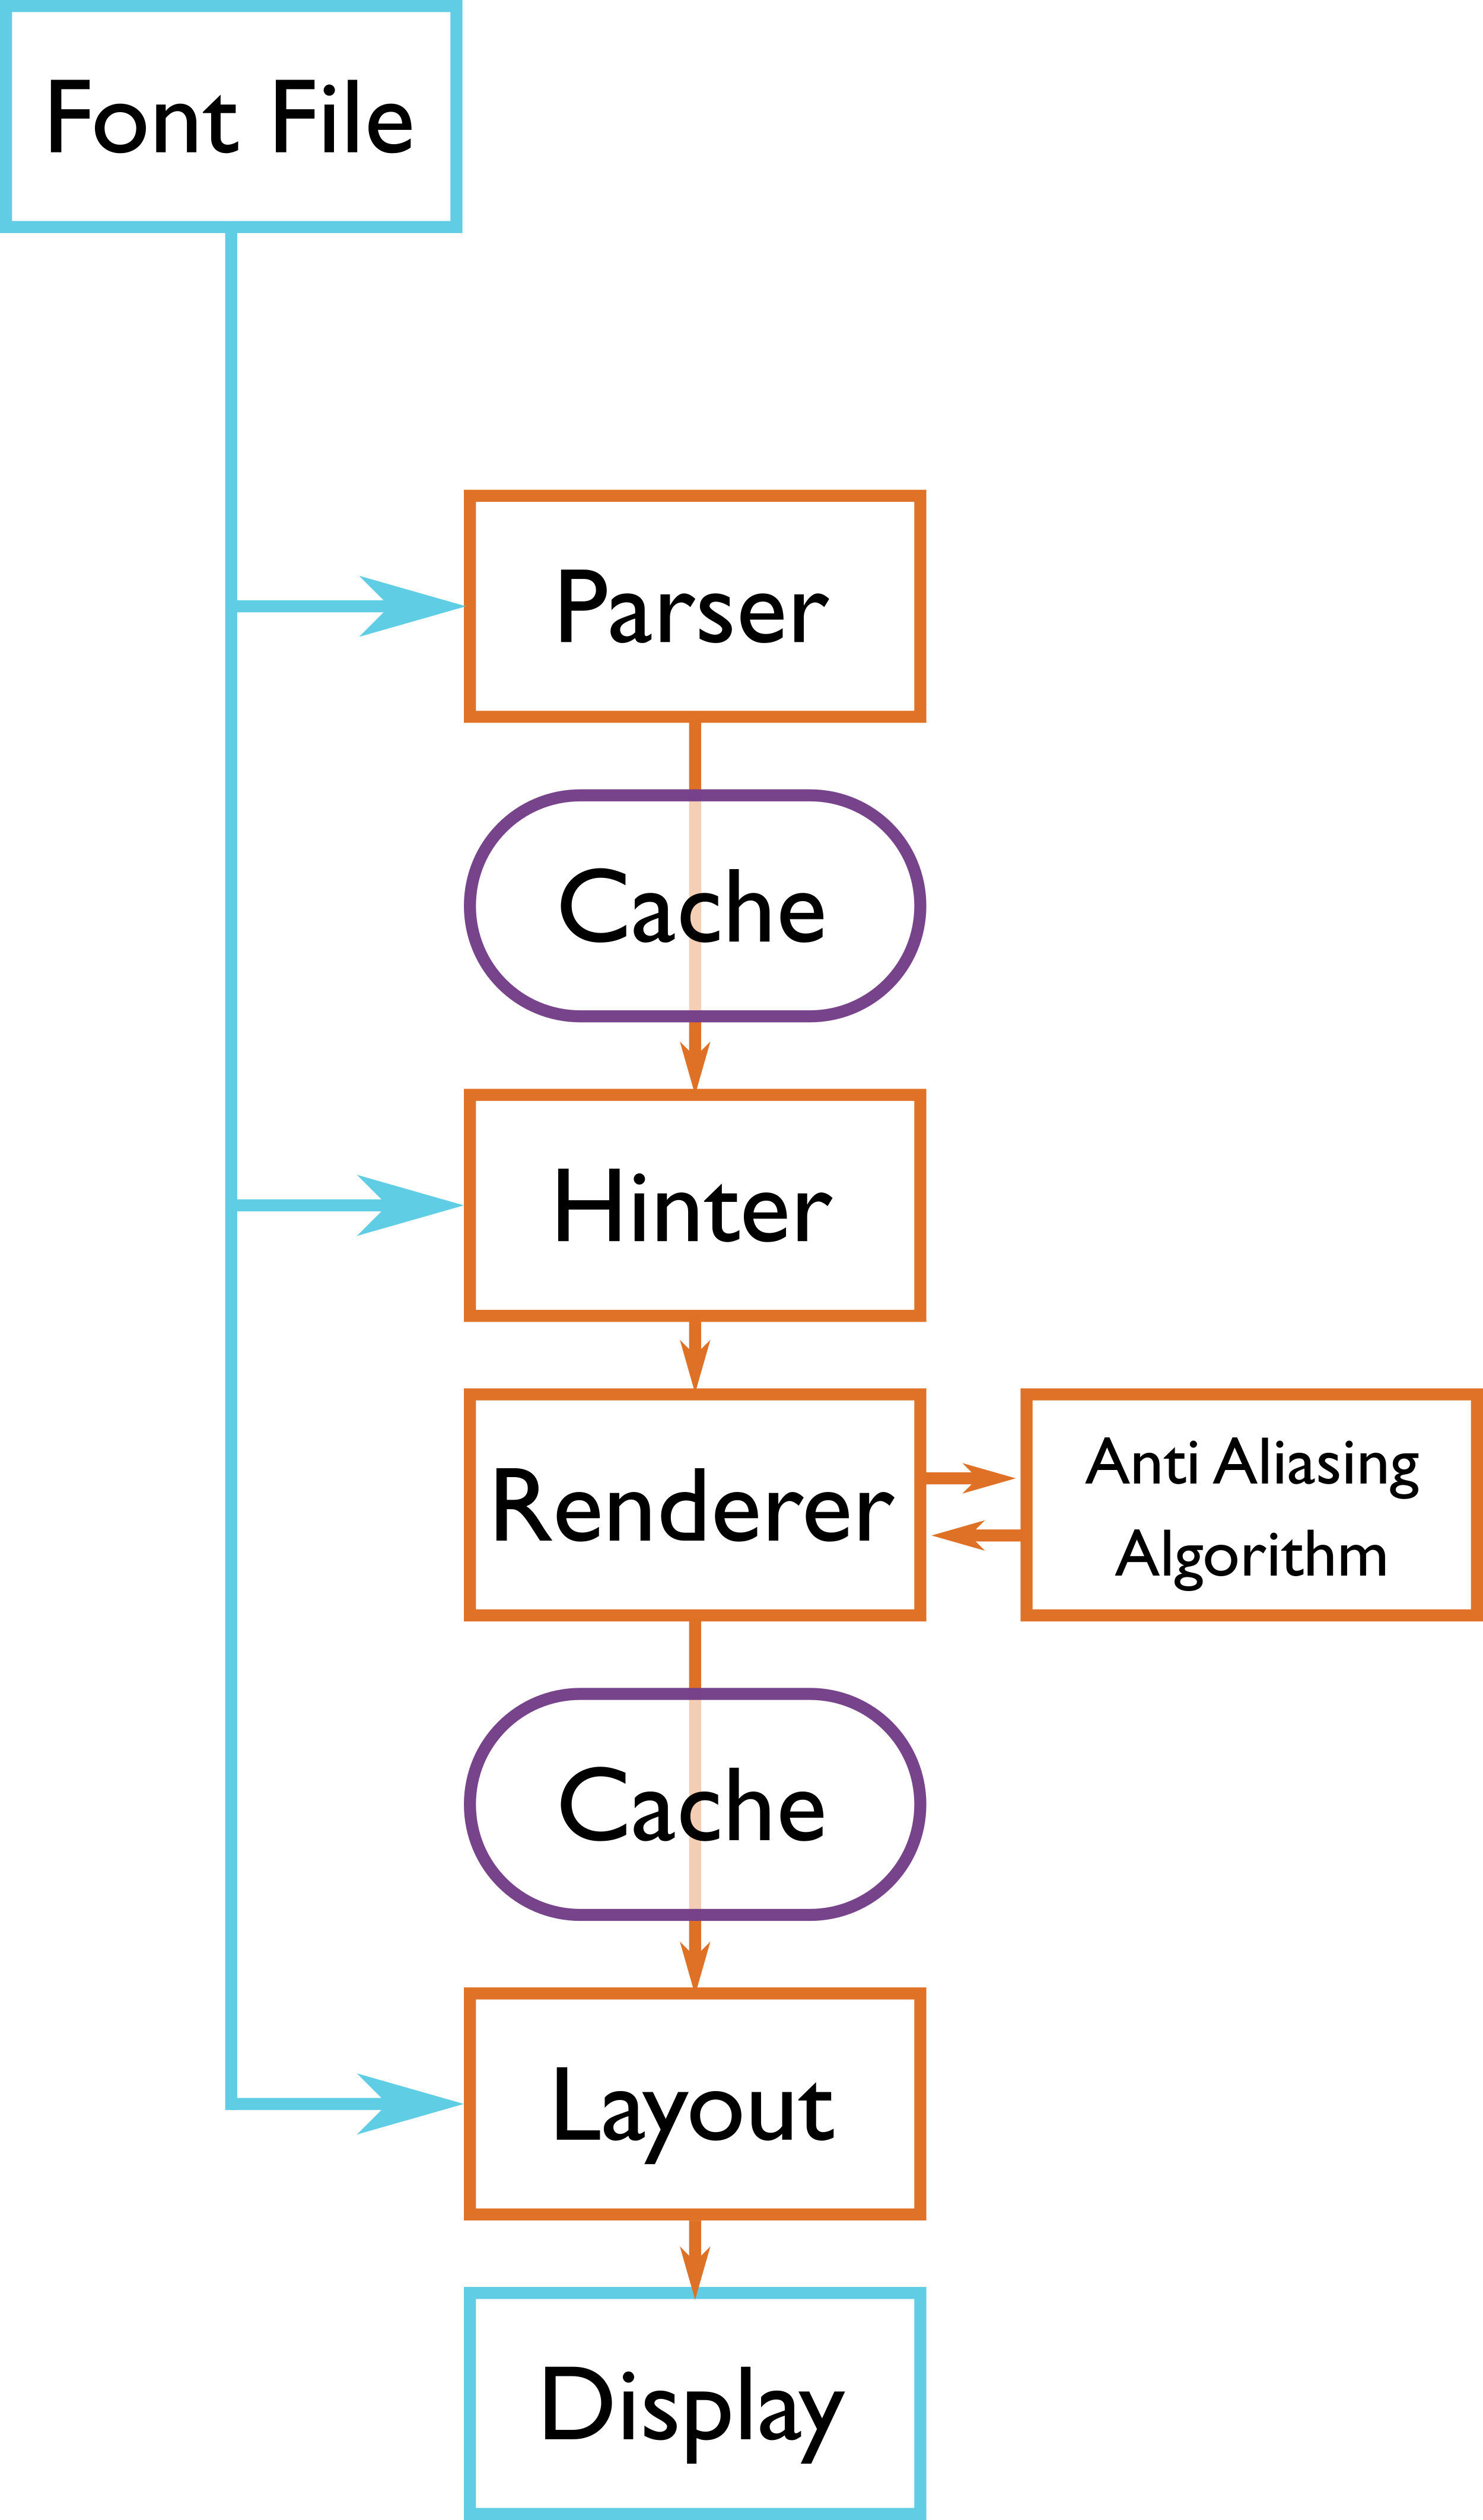
\includegraphics[width=0.4\textwidth]{fontpipelineimg}
\end{wrapfigure}

The hinted font is then rendered, taking the bezier curves of the font and
creating a raster image. This image is then anti-aliased, probably through
supersampling \todo{explain this more}, which is a process that turns a
black-and-white image to a greyscale one which looks sharper on the screen. Some
advanced anti-aliasing techniques take advantage of the RGB format of our
displays, to get a larger effective resolution to work with.

Finally, the anti-aliased image is displayed on the screen. The exact process
behind where it should be placed is handled by a layout engine, which is
responsible for forming individual glyphs into words and pages. A layout engine
still needs to reference the original font file, as kerning information which
dictates the individual spacing between characters is stored in a table there.

font file \rightarrow parser \rightarrow cache \rightarrow hinting \rightarrow
rendering \rightarrow anti-aliasing \rightarrow layout


\subsection{The TrueType Format}
A TrueType font file is a binary file that contains all the data needed to
display a font on the screen. The format, initially codenamed `Bass', was
designed by Apple in the 1980s for Mac System 7, and has continued to evolve and
is now used by virtually every consumer operating system and font engine. The
full specification is available at
\url{https://developer.apple.com/fonts/TrueType-Reference-Manual/}, which will
be summarized here.

A TrueType font is identified by the magic bytes (the first few bytes of many
file formats are different to aid in distinguishing them) \texttt{0x00010000}.
This is followed by a table directory which provides offsets to the various
tables used in the file. Each table contains some information about how the font
should be rendered, or metadata such as the font licence or author. For example,
the \texttt{kern} table contains data related to font kerning, which controls
the spacing between individual letters.

There are several mandatory tables, as shown below. More tables may exist in the
file, but are optional, and may contain extensions to the format, or other data
such as raster images.
\begin{center}
  \begin{tabular}{ l | l }
    
    Name & Function \\
    \hline
    \texttt{cmap} & Maps between characters and glyphs \\
    \texttt{glyf} & Stores the actual glyph data \\
    \texttt{head} & Font header, contains various data involved in the rest of the font \\
    \texttt{hhea} & Secondary header containing specifics of horizontal font layout \\
    \texttt{hmtx} & Data on the metrics of fonts when layed out horizontally \\
    \texttt{loca} & Indexes glyph IDs to offsets in the file \\
    \texttt{maxp} & Contains the maximum quantities of various features of the font \\
    \texttt{name} & Contains the name of the font \\
    \texttt{post} & Data for printing fonts \\
  \end{tabular}
\end{center}

The tables of relevance to this project are \texttt{head}, \texttt{loca},
\texttt{cmap}, and \texttt{glyf}. A detailed explanation of table data
structures can be found in the TrueType specification; a simplified version of
the \texttt{glyf} table is shown below:

The \texttt{glyf} table consists of a number of glyph data structures. Each data
structure is either a simple or compound glyph, and is of the form

\begin{bytefield}[bitwidth=2.2em]{16}
  \bitheader{0-15} \\
  \begin{rightwordgroup}{Glyph header}
    \wordbox{1}{numberOfContours} \\
    \bitbox{16}{xMin} \\
    \bitbox{16}{xMax} \\
    \bitbox{16}{yMin} \\
    \bitbox{16}{yMax} 
  \end{rightwordgroup} \\

  \wordbox{3}{Either a simple glyph data structure, or a compound glyph data
    structure, dependent on the value of \texttt{numberOfContours}.}
\end{bytefield}
\\

\begin{bytefield}[bitwidth=2.2em]{16}
  \bitbox{16}{\textbf{Simple Glyph Data}} \\
  \bitheader{0-15} \\
  \wordbox{2}{Array of glyph contour endpoints, one word wide,
    \texttt{numberOfContours} long.} \\
  \wordbox{1}{instructionLength} \\
  \bitbox{8}{Instruction 1} & \bitbox{8}{Instruction 2} \\
  \bitbox{8}{Instruction 3} & \bitbox{8}{...} \\
  \bitbox{8}{...} & \bitbox{8}{Instruction $n$} \\
  \wordbox[tlr]{3}{Array of flags, length can be determined from the final
    endpoint index} \\
  \bitbox[l]{8} {Example:} & \bitbox{1}{C} & \bitbox{1}{xSh} & \bitbox{1}{ySh} &
  \bitbox{1}{R} & \bitbox{1}{xR} & \bitbox{1}{yR} & \bitbox{2}{Reserved} \\
  \wordbox[blr]{1}{}\\
  \wordbox{2}{Array of deltaX}\\
  \wordbox{2}{Array of deltaY}\\
  \\
  \\
  \bitbox{16}{\textbf{Compound Glyph Data}}\\
  \bitheader{0-15} \\
  \wordbox{1}{Flags (see full spec for details)}\\
  \wordbox{1}{Glyph Index}\\
  \wordbox{2}{\textit{variable size}\\Argument 1 (flag dependent)}\\
  \wordbox{2}{\textit{variable size}\\Argument 2 (flag dependent)}
\end{bytefield}

\textit{Note: Most uses of compound glyph tables are outside of the scope of this project.}
\\
\\

To turn a character into a set of points, we must first lookup the character in
the \texttt{cmap} table. This will give us a glyph index, which we can index
into the \texttt{loca} table to get a glyph offset and length. Finally, we can
use the offset and length to find the appropriate section of the \texttt{glyf}
table, and get the glyph data itself.

\section{Project Objectives}
\begin{enumerate}
  \item{The program will parse TTF files correctly, extracting character and
      glyph data from them.}
  \item{The program will display single characters on the screen in a specified
      font.}
  \item{The program will display these characters in a reasonable amount of
      time, say, not longer than a second (1000ms)}
  \item{The program will anti-alias these characters for improved readability}
  \item{The program will reject incorrectly formed TTF files in a safe manner}
\end{enumerate}

\chapter{Design}
\section{High Level Design}

\begin{wrapfigure}{r}{0.5\textwidth}
  \centering
  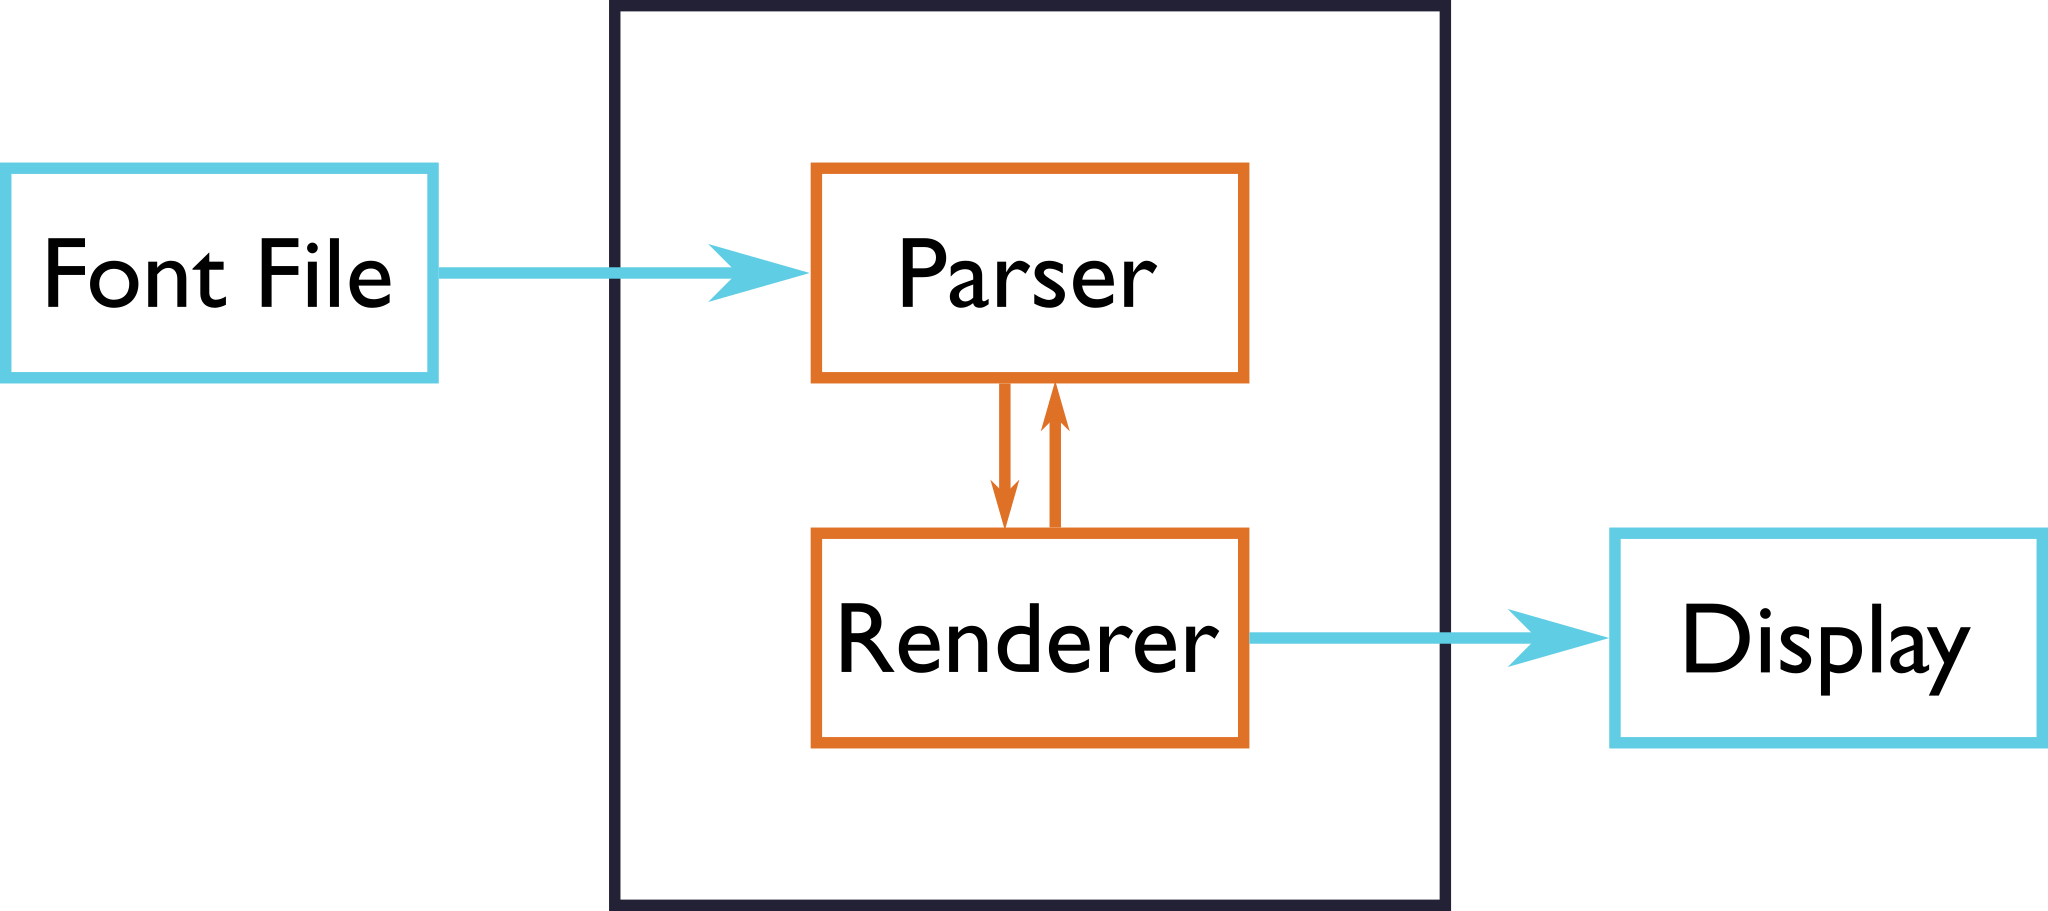
\includegraphics[width=0.5\textwidth]{design/highlevelout}
\end{wrapfigure}

The task has 2 clear subdivisions:
\begin{enumerate}
\item{Parsing the specified font file.}
\item{Displaying the parsed bezier curves on the screen.}
\end{enumerate}


I anticipate task 1 being the hardest, because the TrueType format is very
complex and requires sophisticated parsing to extract the data needed. In
contrast, rendering bezier curves to the screen is a task is moderately simple,
as the bezier curve is used frequently in computer graphics applications.

I will program in C++, using the cmake build system, and use the SDL graphics
library to display the rendered characters to the screen. Finally, I will use a
slightly modified version of \texttt{sdl\_gfx} to make rendering the characters easier. 

\subsection{The Parser}
The parser needs to take the filename of a font, and by examining the associated
file, read various data about the font. The following is a loose list of the
data needed; other data may be needed to properly parse this, or for other
purposes.

\begin{enumerate}
  \item{The \texttt{head} table, which contains information about the rest of
      the file}
  \item{The \texttt{cmap} table, which contains the mapping between character
      and glyph index}
  \item{The \texttt{loca} table, which maps glyph indices to offsets from the
      start of the \texttt{glyf} table}
  \item{The individual glyph data, which requires the above data points to
      find in the file}
  \item{Various font metrics, contained in various tables around the font file}
\end{enumerate}

At the very beginning of the file is the table directory, which contains the
locations and length of all the font tables. Parsing this allows us to look up
the locations of the rest of the data in the file. Next we will examine the
\texttt{head} table to store important metrics that will be used elsewhere in
the file.

At this point, the program will prompt the user for the character that they
would like displayed. This character will be looked up in the \texttt{cmap}
table, to get a glyph index, and then the \texttt{loca} table, to convert the
index into a glyph offset and length.

Finally, we lookup the glyph in the \texttt{glyf} table, and store the entire
glyph data structure. This is quite complex to parse, and will have it's own
section of the program specifically. Parsing this will result in a list of
bezier curves to be rendered, which is then passed to the renderer. 

\subsubsection{The \texttt{Font} class}
A key data structure in this project will be the \texttt{Font} class. This is a
large structure that represents a specific font. We create one at the start of
our program, and gradually fill it in over the course of parsing the font. 

\begin{center}
  \begin{tabular}{|p{7.5cm}|c|c|}
    \hline
    \multicolumn{3}{|c|}{The \texttt{Font} class} \\
    \hline
    \textbf{Type} & \textbf{Name} & \textbf{Access} \\
    \hline
    \texttt{Glyph} & glyph & public \\
    \hline
    \texttt{std::string} & filename & private \\
    \hline
    \texttt{Header} & header & private \\
    \hline
    \texttt{HEADTable} & head & private \\
    \hline
    \texttt{CMAPTable} & cmap & private \\
    \hline
    \texttt{std::vector<uint8\_t>*} & data & private \\
    \hline
    \texttt{int} & fileLength & private \\
    \hline
    \texttt{char} & characterToGet & private \\
    \hline
    \texttt{uint32\_t} & glyphOffset & private \\
    \hline
    \texttt{uint32\_t} & glyphLength & private \\
    \hline
    \hline
    \textbf{Signature} & \textbf{Returns} & \textbf{Access} \\
    \hline
    \texttt{Font()} & Font & public \\
    \hline
    \texttt{Font(std::string filename, char characterToGet)} & Font & public \\
    \hline
    \texttt{readFont(std::string filename)} & void & private \\
    \hline
  \end{tabular}
\end{center}

The most important section of this class is the \texttt{readFont} method. It is
called in the constructor of the font, and does the following things:

\begin{enumerate}
\item Opens the file speficied by \texttt{filename}.
\item Reads that file into the \texttt{data} variable in memory.
\item Parses the header of the font to get the offsets of the tables.
\item Parses the HEAD table into the the \texttt{head} variable.
\item Parses the CMAP table into the \texttt{cmap} variable.
\item Uses the \texttt{cmap} table to get the glyph index of the requested glyph.
\item Looks up this glyph index in the \texttt{loca} table.
\item Parses the glyph using that information. 
\end{enumerate}

This prepares the font to be passed to the renderer, where the public member
\texttt{glyph} will be read by the renderer itself to draw the font to the screen.

\subsubsection{Parsing Fonts}

The TTF specification uses a number of different types of data, which must be
parsed from a series of bytes. My project has a utility module that contains
various functions to take a data array and an offset, and can return a requested
data type from that data. For example, \texttt{parse16} will return a signed 16-bit
integer parsed from the bytes after the offset given. These functions are used
throughout the project, and the util module is included in nearly every file of
the parsing system.

\subsubsection{The Glyph Table}

The core algorithm of the parsing section is the glyph parser. To save space,
data in the glyph itself is not repeated, instead a special flag is set to tell
the parser to repeat this data again. In addition, we must calculate when to
switch from parsing x values to parsing y values, which requires special
calculations to do. The algorithm in pseudocode is as follows:

\begin{Verbatim}[numbers=left]
Glyph::parse(data, offset, length):
  numberOfContours = parse an unsigned 16bit integer at (offset)
  xMin = parse an unsigned 16bit integer at (offset+2)
  yMin = parse an unsigned 16bit integer at (offset+4)
  xMax = parse an unsigned 16bit integer at (offset+6)
  yMax = parse an unsigned 16bit integer at (offset+8)

  if numberOfContours < 0:
    abort() (compound glyphs are outside the scope of the program)

  endPointsOfContours = empty vector
  for (i = 0; i < numberOfContours; i++):
    parse a 16bit integer at (offset+10+i*2) and append it to   \
    endPointsOfContours

  instructionOffset = offset+10+numberOfContours*2
  instructionLength = parse an unsigned 16bit integer at
                      (instructionOffset)

  dataOffset = instructionOffset + instructionLength
  currentOffset = dataOffset
  
  totalPoints = the last value of endPointsOfContours

  flags = empty vector
  xDeltas = empty vector
  yDeltas = empty vector

  currentOffset += 2
  
  while numberOfPoints < totalPoints:
    construct a PointFlag at the currentOffset and append it to  \
    the flags vector
    numberOfPoints++
    currentOffset++

  currentOffset--

  for each flag in flags:
    xDelta = 0
    if xShortVector is set in flag:
      currentOffset++
      xDelta = parse an unsigned 8bit integer at (currentOffset)
      if sign is not set in flag:
        xDelta = -xDelta
    else:
      if xSame is not set in flag:
        currentOffset++
        xDelta = parse a signed 16bit integer at (currentOffset)
        currentOffset++
      else: (if xSame is set)
        xDelta = 0 
    append xDelta to xDeltas

  repeat the above loop for the yDeltas

  for each i in range(length(xDeltas)):
    point = (xDelta, yDelta, flag)
    append point to points

  return points
\end{Verbatim}

\todo{EXPLAIN THIS PROPERLY}

\subsection{Rendering}

The rendering system is comparitively much simpler. We take the points array
returned by the algorithm above, and draw it to the screen. To make this process
simpler, we use a slightly modified version of the \texttt{sdl\_gfx} library.
This library has been modified to allow for anti-aliased bezier curves, which
previously the library did not support. 

First, we iterate through the list of points to convert all of the delta values
into absolute coordinates. During this process, we also insert phantom points
between two off-curve points, to allow the drawing routine to look at the points
in sets of two or three. Finally, we add the first point again at the end of the
loop, to ensure that the loop gets closed.

Now that we have prepared our final list of points, we iterate through each
point, drawing either a line or a bezier curve (using the \texttt{sdl\_gfx}
library functions) as required. These are drawn onto the back framebuffer, which
is then made the active framebuffer (and displayed on the screen) with the call
to \texttt{SDL\_RenderPresent} in \texttt{main()}.

\chapter{Technical Solution}




\end{document}